\input{../../doc_pdf}
\input{../../preamb_pdf}
\usepackage{xr}
\externaldocument{../../bokR2_PDF}

\begin{document}
\textit{Så lenge ikke annet er nevnt, tas det for gitt at $ n\in \mathbb{Z} $.} \vsk

\opr{rads}\\
\textbf{a)}
\algv{
60^\circ &= \frac{60\pi}{180}\br
&= \frac{\pi}{3}
}
\textbf{b)}
\algv{
	15^\circ &= \frac{15\pi}{180}\br
	&= \frac{\pi}{12}
}
\opr{grad}\\
\textbf{a)}
\algv{
	\frac{11\pi}{12} &= \frac{11\pi}{12}\cdot\frac{180}{\pi}^\circ\br
	&= 165^\circ
}
\textbf{b)}
\algv{
	\frac{11\pi}{6} &= \frac{11\pi}{6}\cdot\frac{180}{\pi}^\circ\br
	&= 330^\circ
}

\opr{pytg}\\
I enhetssirkelen er $ |\cos x| $ og $ |\sin x| $ katetene i en rettvinklete trekant med en hypotenus med lengde lik 1. Av Pygagoras' setning får man da at:
\alg{
|\cos x|^2 + |\sin x|^2 =1\\
\cos^2 x + \sin^2 x = 1
}

\opr{tanx}\\
\textbf{a)} \algv{\tan x&= \frac{\sin x}{\cos x} \br
&= \frac{0}{1} \\
&= 0}
\newpage
\textbf{b)} \algv{\tan x& = \frac{\frac{1}{2}}{-\frac{\sqrt{3}}{2}} \br
	&= -\frac{1}{2}\cdot\frac{2}{\sqrt{3}} \br
&= -\frac{1}{\sqrt{3}}}

\opr{bruk1}\\
Vi har at:
\alg{
\cos^2\left(\frac{\pi}{6}\right) + \sin^2\left(\frac{\pi}{6}\right)  &= 1\\
\sin^2\left(\frac{\pi}{6}\right) &= 1-\left(\frac{\sqrt{3}}{2}\right)^2 \\
\sin^2\left(\frac{\pi}{6}\right) &= 1- \frac{3}{4} \\
\sin\left(\frac{\pi}{6}\right) &= \pm\sqrt{\frac{1}{4}}\\
&= \pm\frac{1}{2}
}
Siden $ \frac{\pi}{6} $ ligger i første kvadrant, må sinusverdien være positiv, og altså lik $ \frac{1}{2} $.\vsk

\opr{sin2xopg}\\
\textbf{a)} Vi legger merke til at $ {2x=x+x} $, av \eqref{suv} har vi da at:
\alg{
\sin(2x) &= \sin(x+x) \\
&= \sin x \cos x + \cos x \sin x \\
=& 2 \cos x \sin x
}
\textbf{b)} 
\algv{
2\cos \left(\frac{\pi}{12}\right)\sin \left(\frac{\pi}{12}\right)&=
\sin\left(\frac{\pi}{6}\right)\\ &= \frac{1}{2} }

\opr{cossomsin} \\
Vi legger til og trekker ifra $ \frac{\pi}{2} $ i argumentet:
\[ \cos\left(3x-\frac{7\pi}{2}\right) = \cos\left(3x-\frac{7\pi}{2}+\frac{\pi}{2}-\frac{\pi}{2}\right) \]
Fra (\ref{cossomsi}) har vi da at:
\alg{\cos\left(3x-\frac{7\pi}{2}+\frac{\pi}{2}\right) &= \sin\left(3x-\frac{7\pi}{2}+\frac{\pi}{2}\right) \\
&= \sin(3x + 2\pi) \\
&= \sin(3x)}

\opr{cossinsin}\\
Av (\ref{rsin}) vet vi at vi kan skrive:
\alg{f(x) = r \sin(2x + c) }
hvor $ r $ er gitt som:
\algv{
	r &= \sqrt{1^2+\sqrt{3}^2} \\
	&= 2
}
mens $ c $ er gitt ved ligningssettet: 
\algv{\cos c &=\frac{\sqrt{3}}{2} \br
	\sin c &= \frac{1}{2}}
En $ c $ som oppfyller dette er $ c = \frac{\pi}{6} $.

Altså får vi:
\[ \cos( 2x) + \sqrt 3\sin (2x) =2 \sin\left(2x+\frac{\pi}{6}\right) \]

\opr{sincos0}\\
\textbf{a)} Siden $ \acos 0 = \frac{\pi}{2} $ har vi fra (\ref{coslig}) at:
\[ x = \frac{\pi}{2}+2\pi n\quad \vee \quad -\frac{\pi}{2}+2\pi n \]
Men siden $ n $ er et vilkårlig heltall, kan vi alltids trekke ut $ 2\pi $ fra leddet $ 2\pi n $ uten at løsningen er forandret. Gjør vi dette kan vi skrive:
\alg{
	-\frac{\pi}{2} + 2\pi n &= -\frac{\pi}{2} + \pi+\pi + 2\pi n \br
	&= \frac{\pi}{2} + \pi(2n+1)
}
Vi ser da at vi kan skrive de to løsningene som $ \frac{\pi}{2} $ pluss enten et partalls antall $ \pi $ eller et oddetalls antall $ \pi $. Altså  kan vi skrive begge løsningene kombinert som $ \frac{\pi}{2} $ pluss alle heltalls antall $ \pi $:
\[ x = \frac{\pi}{2}+\pi n \]
\textbf{b)} Siden $ \asin 0 = 0 $ har vi fra (\ref{sinlig}) at:
\[ x = 2\pi n \quad\vee\quad x=\pi +2\pi n \]
Men siden $ x=\pi + 2\pi=\pi(2n+1) $, kan vi med samme argumentasjon som i opg. a) skrive:
\[ x = \pi n \]
\opr{triligns}\\
\textbf{a)} \alg{
\cos x&=\frac{\sqrt{2}}{2} \\
x&= \pm \frac{\pi}{4}+2\pi n
}
\textbf{b)} Av opg. \ref{sincos0} a) vet vi at:
\alg{
\frac{\pi}{3}x &= \frac{\pi}{2}+\pi n \\
x &= \frac{3}{2}(1+2 n)
}
Faktoriseringen av uttrykket over gjør det lettere å identifisere hvilke $ x $ som ligger i intervallet $ [0, 5] $. Dette er $ x=\frac{3}{2} $ og $ x = \frac{9}{2} $. \vsk

\textbf{c)} \algv{
	2\sin(3x) &=1 \\
	\sin(3x)&= \frac{1}{2} \\
}
Vinklene $ \frac{\pi}{6} $ og $ \frac{5\pi}{6} $ har sinusverdien $ \frac{1}{2} $, altså har vi at:
\alg{
3x &= \frac{\pi}{6} +2\pi n \\
x &= \frac{1}{3}\left(\frac{\pi}{6}+2\pi n\right)
}
eller at:
\alg{
	3x &= \frac{5\pi}{6} +2\pi n \\
	x &= \frac{1}{3}\left(\frac{5\pi}{6}+2\pi n\right)
}
\textbf{d)} Siden $ -\frac{\pi}{3} $ og $ -\frac{2\pi}{3} $ har sinusverdien, har vi at:
\alg{
2x-\pi &= -\frac{\pi}{3}+2\pi n \\
x &= \frac{1}{2}\left(\frac{2\pi}{3}+2\pi n\right) \\
&= \frac{\pi}{3}(1+3n)
}
eller at:
\alg{
	2x-\pi &= -\frac{2\pi}{3}+2\pi n \\
	x &= \frac{1}{2}\left(\frac{\pi}{3}+2\pi n\right) \\
	&= \frac{\pi}{6}(1+6n)
}
\textbf{e)} \algv{
2\sqrt{3}\tan \left(4x+\frac{\pi}{2}\right) &= 2 \\
\tan \left(4x+\frac{\pi}{2}\right) &= \frac{1}{\sqrt{3}}
}
Siden $ \frac{\pi}{6} $ har $ \frac{1}{\sqrt{3}} $ som tangensverdi, har vi at:
\alg{
4x+\frac{\pi}{2} &= \frac{\pi}{6}+\pi n\\
x &= \frac{1}{4}\left(\pi n-\frac{\pi}{3}\right)
}
\opr{asinbcos0o}\\
\textbf{a} \algv{
	\sqrt{3} \sin x - \cos x &=0 \\
	\frac{\sqrt{3}\sin x}{\cos x} &= \frac{\cos x}{\cos x}\\
	\tan x &= \frac{1}{\sqrt{3}}\\
	x &= \frac{\pi}{6}+\pi n
}

\textbf{b)} \algv{
	\sin x + \sqrt{3}\cos x &=0 \\
	\frac{\sin x}{\cos x} &= -\sqrt{3} \br
	\tan x &= -\sqrt{3} \\
	x &= -\frac{\pi}{3}+\pi n
}

\textbf{c)} \algv{
\cos (2x) + \sin (2x)=&0 \\
\tan (2x) &= -1 \\
2x &= -\frac{\pi}{4}+\pi n \\
x &= \frac{1}{2}\left(\pi n-\frac{\pi}{4}\right)
}

\opr{kombo}\\
\textbf{a)}  Vi omskriver ligningen til sinusligningen
\alg{
	r\sin(x+c)&= \sqrt{2}
}
hvor:
\alg{r &= \sqrt{1^2+1^2} \\
	&= \sqrt{2}
}
og der $ c $ oppfyller ligningssettet:
\alg{
	\cos c &= \frac{1}{\sqrt{2}} \br
	\sin c &=  \frac{1}{\sqrt{2}}
}
$ c=\frac{\pi}{4} $ oppfyller kravene over \big($ {\frac{1}{\sqrt{2}}=\frac{2}{\sqrt{2}\sqrt{2}}=\frac{\sqrt{2}}{2}} $\,\big), altså får vi:
\alg{\sqrt{2}\sin\left(x+\frac{\pi}{4}\right) &= \sqrt{2} \br
 \sin\left(x+\frac{\pi}{4}\right)  &= 1
}
Altså må:
\algb{
x+\frac{\pi}{4}&= \frac{\pi}{2}+2\pi n \\
x &= \frac{\pi}{4}+2\pi n
}

\textbf{b)} Vi omskriver ligningen til sinusligningen
\alg{
	r\sin\left(\frac{x}{2\pi}+c\right)&= 1
}
hvor:
\alg{r &= \sqrt{\sqrt{3}^2+(-1)^2} \\
	&= 2
}
og der $ c $ oppfyller ligningssettet:
\alg{
	\cos c &= -\frac{1}{2} \br
	\sin c &= \frac{\sqrt{3}}{2}
}
$ c=\frac{2\pi}{3} $ oppfyller kravene over, altså får vi:
\alg{2\sin\left(\frac{x}{2\pi}+\frac{2\pi}{3}\right) &= 1 \br
	\sin\left(\frac{x}{2\pi}+\frac{2\pi}{3}\right) &= \frac{1}{2} 
}
Vi må altså enten ha at:
\alg{\frac{x}{2\pi}+\frac{2\pi}{3} &= \frac{\pi}{6}+2\pi n \br
	\frac{x}{2\pi}&=-\frac{\pi}{2}+2\pi n\br
	x &= \pi^2(4n-1) }
eller at:
\alg{\frac{x}{2\pi}+\frac{2\pi}{3} &= \frac{5\pi}{6}+2\pi n \br
	\frac{x}{2\pi}&=\frac{\pi}{6}+2\pi n\br
	x &= 2\pi\left(\frac{\pi}{6}+2\pi n\right) }

\opr{abctri}\\
\textbf{a)} Vi løser andregradsligningen mhp. $ \sin x $, og får at:
\[ \sin x = \frac{1}{2}\quad\vee\quad x= -1 \]
I tilfellet av at $ {\sin x = \frac{1}{2}} $, må:
\[ x = \frac{\pi}{4}+2\pi n\quad\vee\quad \frac{3\pi}{4}+2\pi n \]
I tilfellet av at $ {\sin x = -1} $, må:
\[ x = \frac{\pi}{2}+2\pi n\]
\textbf{b)} Vi løser andregradsligningen mhp. $ \cos (3x) $, og får at:
\[ \cos (3x) = -4\quad\vee\quad x= 1 \]
I tilfellet av at $ {\cos (3x) = -4} $ har ligningen ingen reell løsning. I tilfellet av at $ {\cos (3x) = -1} $, må:
\[ x = \frac{\pi +2\pi n}{3}\]
\textbf{c)} Vi løser andregradsligningen mhp. $ \cos x $, og får at:
\[ \cos x = -4\quad\vee\quad x= 1 \]
I tilfellet av at $ {\cos x = -4} $ har ligningen ingen reell løsning. I tilfellet av at $ {\sin x = -1} $, må:
\[ x = 2\pi n\]
\textbf{d)} Vi løser andregradsligningen mhp. $ \tan(\pi x) $, og får at:
\[ \tan(\pi x) = \sqrt{3}\]
Altså må:
\[ x = \frac{1}{3}+n\]

\opr{kvadopg}\\
\textbf{a)} 
\algv{
 -\cos^2 x+15\sin^2 x &= 3(\cos^2 x + \sin^2 x) \\
 12 \sin^2 x &= 4\cos^2 x \\
\frac{ 12 \sin^2 x }{\cos^2 x}&= \frac{4\cos^2 x }{\cos^2 x}\\
12 \tan^2 x &= 4 \\
\tan^2 x &= \frac{1}{3} \\
\tan x &= \pm \frac{1}{\sqrt{3}}
}
Siden $ {\atan \frac{1}{\sqrt{3}}=\frac{\pi}{6}} $ og $ {\atan \left(-\frac{1}{\sqrt{3}}\right)=-\frac{\pi}{6}} $, får vi at:
\[ x = \pm \frac{\pi}{6}+\pi n \]

\textbf{b)} Vi starter med å mulitpliserer ligningen med $ 2 $, og får:
\alg{
2\cos^2 \left(\frac{x}{4}\right) - 4 \sin^2 \left(\frac{x}{4}\right) &= -1 \br
2\cos^2 \left(\frac{x}{4}\right) - 4 \sin^2 \left(\frac{x}{4}\right) &= -1\left(\cos^2\left(\frac{1}{4}\right)+\sin^2\left(\frac{1}{4}\right)\right) \br
- 3 \sin^2 \left(\frac{x}{4}\right)&= -3\cos^2 \left(\frac{x}{4}\right) \br
\tan^2 \left(\frac{x}{4}\right)&= 1 \br
\tan \left(\frac{x}{4}\right) &= \pm 1
}
Siden $ \atan 1 = \frac{\pi}{4} $ og $ \atan (-1) = -\frac{\pi}{4} $, får vi at:
\alg{
\frac{x}{4} &= \pm \frac{\pi}{4}+\pi n \\
x&= \pm \pi + 4\pi n
}
Det er helt greit slå seg til ro med svaret over (på en eksamen vil dette gi full uttelling), men vi skal likevel foreta en operasjon som gjør at uttrykket blir enda mer kompakt:\vsk

Siden vi av leddet $ 4\pi n $ kan trekke ut så mange multiplum av $ 4\pi $ vi måtte ønske, kan vi for løsningen hvor $ \pi $ har negativt fortegn skrive:
\alg{x &= -\pi + 4\pi + 4\pi n \\
x &= \pi +2\pi + 4\pi n \\
&= \pi +2\pi(2n+1)
}
Videre utfører vi en enkel faktorisering av løsningen der $ \pi $ er positiv:
\[ x=\pi+ 2\pi(2n) \]
Av de to uttrykkene over innser vi at $ x $ kan skrives som $ \pi $ pluss $ 2\pi $ ganget med et vilkårlig oddetall eller et vilkårlig partall, altså alle heltall! Derfor får vi at:
\[ x = \pi +2\pi n \]

\opr{cosmaks}\\
\textbf{a)} Når $ a>0 $ må $ f $ må ha sin største verdi når cosinusverdien er lik 1, altså når:
\[ \cos(kx + c) = 1 \]
Av (\ref{coslig1}) får vi da at:
\[ kx +c = 2\pi n \]
Videre må $ f $ ha sin minste verdi når cosinusverdien er lik $ -1 $, altså når:
\[ \cos(kx + c) = -1 \]
Av (\ref{coslig_1}) får vi da at:
\[ kx +c = 2\pi n \]

\textbf{b)} Når $ a<0 $ får vi bare det omvendte av situasjonen i opg. a).\vsk

\opr{cosfunko}\\
\textbf{a)}
Perioden $ P $ finner vi av relasjonen:
\[ k = \frac{2\pi}{P}  \]
som gir:
\algv{
P &= \frac{2\pi}{k}\br
&= \frac{2\pi}{3}
}
\textbf{b)} Maksimumsverdien $ f_{maks} $ er amplituden addert med konstantleddet:
\alg{f_{maks}&=5+4 \\
&= 9
}
Minimumsverdien $ f_{min} $ er konstandleddet fratrekt amplituden:
\alg{f_{min}&=4-5 \\
	&= 2
}
\textbf{c)} $ f $ må ha sitt maksimum når cosinusverdien blir $ -1 $, dette skjer når:
\alg{3x+\frac{\pi}{12} &= \pi +2\pi n \br
	3x &=  \pi-\frac{\pi}{12}+2\pi n \br 
	x &= \frac{1}{3}\left(2\pi n-\frac{\pi}{12}\right)
}
Videre må $ f $ ha sitt minimum når cosinusverdien blir $ 1 $, altså når:
\alg{3x+\frac{\pi}{12} &= 2\pi n \br
	3x &= 2\pi n -\frac{\pi}{12} \br
	x &= \frac{1}{3}\left(2\pi n-\frac{\pi}{12}\right)
}

\opr{sinmaks}\\
\textbf{a)} Når $ a>0 $ må $ f $ må ha sin største verdi når sinusverdien er lik 1, altså når:
\[ \sin(kx + c) = 1 \]
Av (\ref{sinlig1}) får vi da at:
\[ kx +c = \frac{\pi}{2}+ 2\pi n \]

Videre må $ f $ ha sin minste verdi når sinusverdien er lik $ -1 $, altså når:
\[ \sin(kx + c) = -1 \]
Av (\ref{sinlig_1}) får vi da at:
\[ kx +c = -\frac{\pi}{2}+2\pi n \]

\textbf{b)} Når $ a<0 $ får vi bare det omvendte av situasjonen i opg. a).\vsk 

\opr{sinfnpkt}\\
\textbf{a)} \algv{
P &= \frac{2\pi}{k} \br
&= \frac{2\pi}{\frac{\pi}{2}} \br
&= 4
}
\textbf{b)} $ f $ har maksimumspunkter der hvor sinusverdien er lik $ -1 $, altså når:
\alg{ 
	\frac{\pi}{2} x &= -\frac{\pi}{2}+2\pi n\\
	x &= 4 n-1
}
På intervallet $ x\in[-3, 3] $ vil $ x=-1 $ og $ x=3 $ oppfylle ligningen over. $ f_{maks} $ vil i alle tilfeller være lik 3, derfor blir toppunktene $ (-1, 3) $ og $ (3, 3) $.\vsk

\textbf{c)} \alg{
-2\sin\left(\frac{\pi}{2}x\right) +1&=0  \br
\sin\left(\frac{\pi}{2}x\right) &= \frac{1}{2}\br
}
Av (\ref{sinlig}) kan vi enten ha at:
\alg{\frac{\pi}{2}x &= \frac{\pi}{6}+2\pi n \br
	x &= \frac{1}{3}(1+12n)}
eller at:
\alg{\frac{\pi}{2}x &= \pi-\frac{\pi}{6}+2\pi n \br
	x &= \frac{1}{3}(5+12n)}
På intervallet $ x\in[-3, 3] $ vil $ x=-\frac{7}{3} $, $ x=\frac{5}{3} $ og $ x=\frac{1}{3} $ oppfylle én av de to ligningene over, dette er altså nullpunktene til $ f $.

\textbf{d)} Vi markerer nullpunktene og toppunktene og skisserer sinuskurven som går mellom disse på intervallet $ x\in[-3, 3] $.\vsk

\opr{skissin}\\
Perioden til $ f $ tilsvarer den horisontale avstanden mellom toppunktene, som er $ 2\pi $. Amplituden er vertikalavstanden mellom likevektslinja og toppunktene, som altså er 2. Bunnpunktene ligger en halv bølgelengde unna toppunktene, og siden amplituden er 2, må bunnpunktene ha $ y $-verdien $ 1-2=-1 $.\vds
\begin{figure}
	\centering
	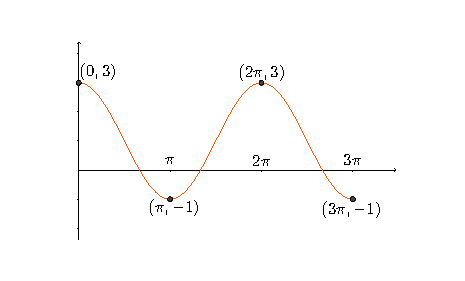
\includegraphics[]{skissin}
\end{figure}

\grubr{opgtangr}
Fordi forholdet $ \frac{a}{b}$ er det samme som $ \frac{\sin x}{\tan x} $, må det finnes et tall $ c $ som er slik at:
\alg{
c\sin x = a \tag{I} \label{gr21}\\
c\cos x = b \tag{II} \label{gr22}
}
Kvadrerer vi begge ligninger og legger dem sammen, får vi:
\alg{
(c\sin x)^2+(c\cos x)^2 &= a^2 + b^2 \\
c^2 &= a^2+b^2 \\
c &= \sqrt{a^2+b^2}
}
Setter vi dette tilbake i \eqref{gr21} og \eqref{gr22}, finner vi at:
\alg{ \sin x &= \frac{a}{\sqrt{a^2+b^2}} \\
\cos x &= \frac{b}{\sqrt{a^2+b^2}}
}
\end{document}